% -------------------------------------------------------------------------
%  This is a good place to outline key components of selected libraries
% -------------------------------------------------------------------------

\section{Selected Amanzi libraries}

This section describes selected Amanzi libraries, their limitations and possible 
ways for extensions.

\subsection{WhetStone}
This library implements primarily local matrices for 
various discretizations frameworks including finite volumes, nonlinear finite volumes,
mimetic finite differences, virtual elements, and discontinuous Galerkin.
Conceptual design of a part of the library is presented in Fig.~\ref{fig:whetstone}.
Classes derived from class {\tt MFD3D} cover a huge spectrum of PDEs.

The library is under extensive development.
At the moment, there exist both a unified approach to discretization schemes of arbitrary
order and the optimized implementation of the low-order schemes.

Additional functionality included in this library supports
\begin{enumerate}
\item the ring algebra of scalar, vector and matrix polynomials;
\item quadrature rules on simplices;
\item numerical integration algorithms based on the Euler homogeneous theorem;
\item coordinate transformations including parameterization of mesh faces and edges.
\end{enumerate}

A few  comments on the design principles. 
Polynomial coefficients are represented by a linear array. 
A polynomial iterator class allow us to access information about monomial terms of 
a given polynomial in a for-type loop:
\begin{lstlisting}
Polynomial poly(3, 2);
for (auto it = poly.begin(); it < poly.end(); ++it) {
  int i = it.PolynomialPosition();
  int k = it.MonomialSetOrder();
  const int* idx = it.multi_index();
  double ci = poly(i);
}
\end{lstlisting}
Each step of this loop extracts information about monomial $c_i \,x^{idx_0} y^{idx_1} z^{idx_2}$
of degree $k= idx_0 + idx_1 + idx_2$ in a quadratic polynomial.

Quadrature rules on simplexes have positive weights for stability of numerical schemes. 
Integration formulas based on Euler's homogeneous theorem can be used for integrating
polynomials over polytopal cells.
To integrate polynomial and non-polynomial functions using a single interface a simple
base class {\tt WhetStoneFunction} is used.

Coordinate transformation allows us to treat a 3D mesh face as a 2D polygon.
This is used in (a) hierarchical construction of high-order virtual element and mimetic 
schemes, and (b) projection of polynomials on a low-dimension manifold and an reserve (non-unique)
lifting operation.

Finally this library contains a factory of discretization schemes that could
be extended by including users schemes via a simple interface.
Example of such an extension is available in directory {\it operators/test}.


\begin{figure}[h!]
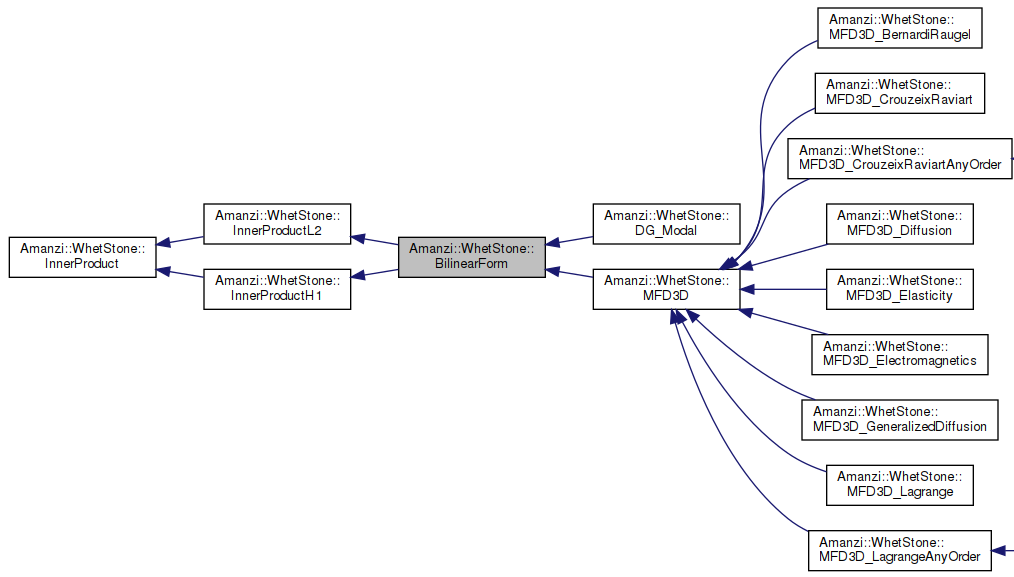
\includegraphics[width=1.0\textwidth]{figs/whetstone.png}
\caption{Partial dependency tree for library WhetStone.\label{fig:whetstone}}
\end{figure}


%%%%%%%%%%%%%%%%%%%%%%%%%%%%%%%%%%%%%%%%%%%%%%%%%%%%%%%%%%%%%%%%%%%%%%
\clearpage
\subsection{Operators}
This is a high-level library that supports global matrices and
various assembly patterns.
Conceptual design of a part of this library is presented in Fig.~\ref{fig:operators}.
Classes derived from a helper class {\tt PDE\_HelperDiscretization} cover 
a range of parabolic and hyperbolic problems.

Additional functionality included in this library supports
\begin{enumerate}
\item cell-based remap schemes;
\item upwind algorithms for cell-centered fields;
\item reconstruction of slopes from cell-based data and their limiting.
\end{enumerate}

To create a preconditioner from an assembled matrix, we need a contiguous vector space.
Two classes {\tt SuperMapLumped} and {\tt SuperMap} in directory {\tt data\_structures} 
takes non-conti\-guous data structures, such as the {\tt CompositeVector} and {\tt TreeVector}
and converts them into a single map.
Unfortunately, un-rolling vectors requires to copy data using functions described in
{\tt OperatorUtils.hh}.

This library was re-factored a few times. 
Implementation of new schemes, most certainly will require an additional re-factory;
however, backward compatibility should be preserved.

\begin{figure}[h!]
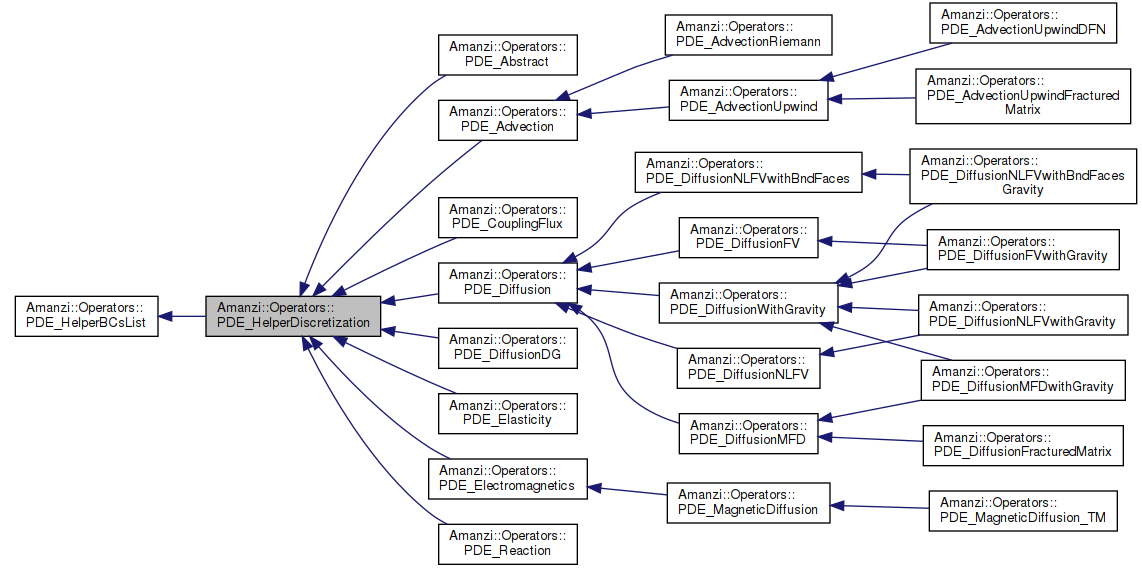
\includegraphics[width=1.0\textwidth]{figs/operators.png}
\caption{Partial dependency tree for library Operators.\label{fig:operators}}
\end{figure}


%%%%%%%%%%%%%%%%%%%%%%%%%%%%%%%%%%%%%%%%%%%%%%%%%%%%%%%%%%%%%%%%%%%%%%
\clearpage
\subsection{Data structures}
This library describes parallel vectors used in Amanzi.
This includes classes {\tt CompositeVector} and {\tt TreeVector} described above.
Additional functionality includes implementation of algorithms that close shortcomings
of various Trilinos interfaces.
For instance, from a user perspective, parallel communications should be the integral 
part of a parallel vector. 
This is done via Amanzi's wrapper classes {\tt CompositeVector} and {\tt TreeVector}.

Classes {\tt GraphFE}, and {\tt MatrixFE} provides capabilities for better assembly 
practices for Epetra-based implementations.
They provide a plausibly scalable matrix for use in FE-like systems, where assembly
must be done into rows of ghost entities as well as owned entities.
These classes uses the "construct, insert, complete fill" paradigm of all
Epetra graphs and CRS matrices.
The only real difference is the use of {\it InserMyIndices()} and {\it SumIntoMyValues()}
which may now take local indices from the ghosted map, not the true row map.


%%%%%%%%%%%%%%%%%%%%%%%%%%%%%%%%%%%%%%%%%%%%%%%%%%%%%%%%%%%%%%%%%%%%%%
\subsection{PKs}
This library provides plausibly abstract classes for implementation of 
boundary conditions and source terms in the physical PKs, see Fig.~\ref{fig:pks}.

Multiple subdirectories contain implementation of various process kernels and MPC PKs.
A PK factory is used for self-registering of PKs from the global input spec.
To register an new PK, the developer must add a private, static member of type 
{\tt RegisteredPKFactory} to the class declaration, and write a special {\tt \_reg.hh} 
file that instantiates the static registry:

\begin{lstlisting}
// pk_implementation.hh
#include "PK.hh"
#include "PK_Factory.hh"
class DerivedPK : public Amanzi::PK {
 private:
  static Amanzi::RegisteredPKFactory<DerivedPK> factory_;
};

// pk_implementation_reg.hh
#include "pk_implementation.hh"
template<>
Amanzi::RegisteredPKFactory<DerivedPK> DerivedPK::factory_("pk unique id");
\end{lstlisting}


Each PK must implement the standard PK interface, as well as interfaces to either 
an explicit time integrator or an implicit solver.
A few comments are below, see the code for the complete description of these interfaces:
\begin{itemize}
\item Function {\it Setup()} is used to create fields (e.g. pressure), field evaluators
      (e.g. water content), and variables (e.g.
      absolute permeability) and to register them with the state.
      This function should avoid any initialization work unless it is really needed
      for the state registration process.

\item Function {\it Initialize()} is used to initialize primary state fields for the PK,
      and miscalleneous structures for discrete PDE operators, time integrators, 
      boundary conditions, source terms, etc.

\item Function {\it AdvanceStep()} is used to advance PK from time one time step to another.
      For an implicit time discretization, it calls an implicit solver.
      For an explicit time discretization, it calls a Runge-Kutta solver or any other ODE
      integrator.

\item Function {\it CommitStep()} is used to update any needed secondary variables at 
      the next time slice under assumption that the time step was sucessful. 

\item Function {\it FunctionalResidual()} is a part of the implict solver interface.
      It computes the non-linear functional at the given solution approximation.

\item Function {\it ModifyPredictor()} is a part of the implict solver interface.
      It modifies optionally the extrapolated guess for the predictor that is going to 
      be used as a starting value for the nonlinear solve in the time integrator.

\item Function {\it FunctionalTimeDerivative()} is a part of the explicit time integration
      interface. It calculates the right-hand side of an ODE system at the given state vector.
\end{itemize}

\begin{figure}[h!]
\begin{center}
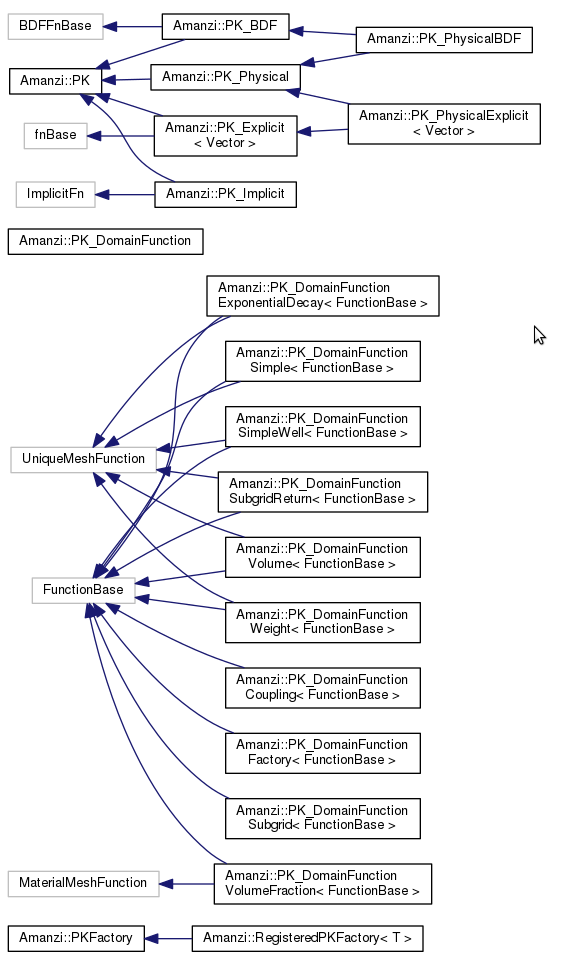
\includegraphics[height=0.9\textheight]{figs/pks.png}
\caption{Partial dependency tree for library PKs.\label{fig:pks}}
\end{center}
\end{figure}


%%%%%%%%%%%%%%%%%%%%%%%%%%%%%%%%%%%%%%%%%%%%%%%%%%%%%%%%%%%%%%%%%%%%%%
\subsubsection{Setup}
The following example shows how to register the evaluator that computes 
the total water content.
First, we define a key for the field to avoid usage of hard-coded names
in the code. 
The key takes a name of a computational domain and the field name.
Next, we populate names of the dependends fields: pressure, saturation,
and porosity.
Finally, we create a secondary variable field evaluator and link it
to the field name.

\begin{lstlisting}
Key wc_key = Keys::getKey(domain, "water_content"); 

S->RequireField(wc_key, wc_key)->SetMesh(mesh)->SetGhosted(true)
  ->SetComponent("cell", AmanziMesh::CELL, 1);

Teuchos::ParameterList elist;
elist.set<std::string>("pressure key", pressure_key_)
     .set<std::string>("saturation key", saturation_liquid_key_)
     .set<std::string>("porosity key", porosity_key_);

auto eval = Teuchos::rcp(new VWContentEvaluator(elist));
S->SetFieldEvaluator(water_content_key_, eval);
\end{lstlisting}
 

%%%%%%%%%%%%%%%%%%%%%%%%%%%%%%%%%%%%%%%%%%%%%%%%%%%%%%%%%%%%%%%%%%%%%%
\subsubsection{Boundary conditions}
To help implementing boundary conditions, this library provides a few helper 
classes derived from the base class {\tt PK\_DomainFunction}.
Each PK has typically its own boundary class derived (optionally) from the
base class, e.g. {\tt FlowBoundaryFunction}.
This class parses the XML sublist {\it boundary conditions} and creates 
distributed arrays with boundary data. The key variable is typically named 
{\it bcs\_} and can be found in a main PK class.
Explicit Transport uses {\it bcs\_} directly.
Other PKs take {\it bcs\_} and populate mesh-size arrays (see class {\tt BCs})
in order to use operators' machinery for imposing boundary conditions.

Another approach to imposing simple boundary condition is useful for unit tests:

\begin{lstlisting}
// get mesh maps with ghosts entities
const auto& fmap = mesh->face_map(true);
const auto& bmap = mesh->exterior_face_map(true);

// loop over boundary faces
for (int bf = 0; bf < bmap.NumMyElements(); ++bf) {
  // local boundary face id -> global face id -> local face id
  int f = fmap.LID(bmap.GID(bf));
  const Point& xf = mesh->face_centroid(f);
  ...
}
\end{lstlisting}




%%%%%%%%%%%%%%%%%%%%%%%%%%%%%%%%%%%%%%%%%%%%%%%%%%%%%%%%%%%%%%%%%%%%%%
\clearpage
\subsection{General purpose factory}
In many cases, the developer may have multiple options that inherit a
common (likely purely) virtual class.  
For instance, many implementations of the equations of state class will 
provide a basic method for $\rho(T,p)$,  including both real "fits" to 
data, analytic expressions, and fake EOS classes for testing. 
We would like to be able to:
\begin{itemize}
\item choose the implementation at run time
\item easily add new implementations
\end{itemize}

To do the first, we use a factory design pattern. 
Like most factories, an implementation must be "registered" with the factory.  
To do the second, this registration must NOT be done in the factory's source code itself.

This is made a little easier by the fact that nearly all of these things
will be constructed using a single interface for the constructor, which
(explicitly) takes a single argument -- a variable of class {\tt ParameterList} -- and
parses that list for its actual parameters.  While it is usually a good
idea to have a factory take the input list, do the parsing, and call the
model's constructor with the parameters, that would require every model
implementation to have its own factory.  To simply things for scientists
writing these models, we choose to do the parsing within the
constructor/initialization.

The obvious exception to this is the model type parameter, which must get
read by a factory and mapped to an implementation's constructor.

The general purpose factory is templated to take a
single base class.  Implementations of that base class then "register"
themselves with the factory instance (which is stored statically since we
cannot correctly manage the cleanup).  This factory assumes all
constructors for all implementations of all base classes take a single
variable of class {\tt ParameterList} as an argument. 
An EOS example:
\begin{lstlisting}
// eos_factory.cc  (no .hh file necessary)
#include "eos.hh" // header for class EOS, a purely virtual base class
#include "factory.hh" // this file
template <> Factory<EOS>::map_type* Factory<EOS>::map_; // explicitly
                                                        // instantiate the
                                                        // static registry
// eos_implementation.hh
#include "eos.hh"
class DerivedEOS : public EOS {
  DerivedEOS(Teuchos::ParameterList& plist);

 private:
  static RegisteredFactory<EOS,DerivedEOS> factory_; // my factory
};

// pk_using_an_eos.cc
#include "eos.hh"

void init(...) {
  Factory<EOS> eos_factory;
  my_eos_ = eos_factory.CreateInstance("my_eos_type", eos_plist);
}
\end{lstlisting}



